\documentclass{standalone}
\usepackage{tikz}
\usetikzlibrary{patterns, positioning}
\usepackage[sfdefault]{ClearSans} %% option 'sfdefault' activates Clear Sans as the default text font
\usepackage[T1]{fontenc}

\begin{document}
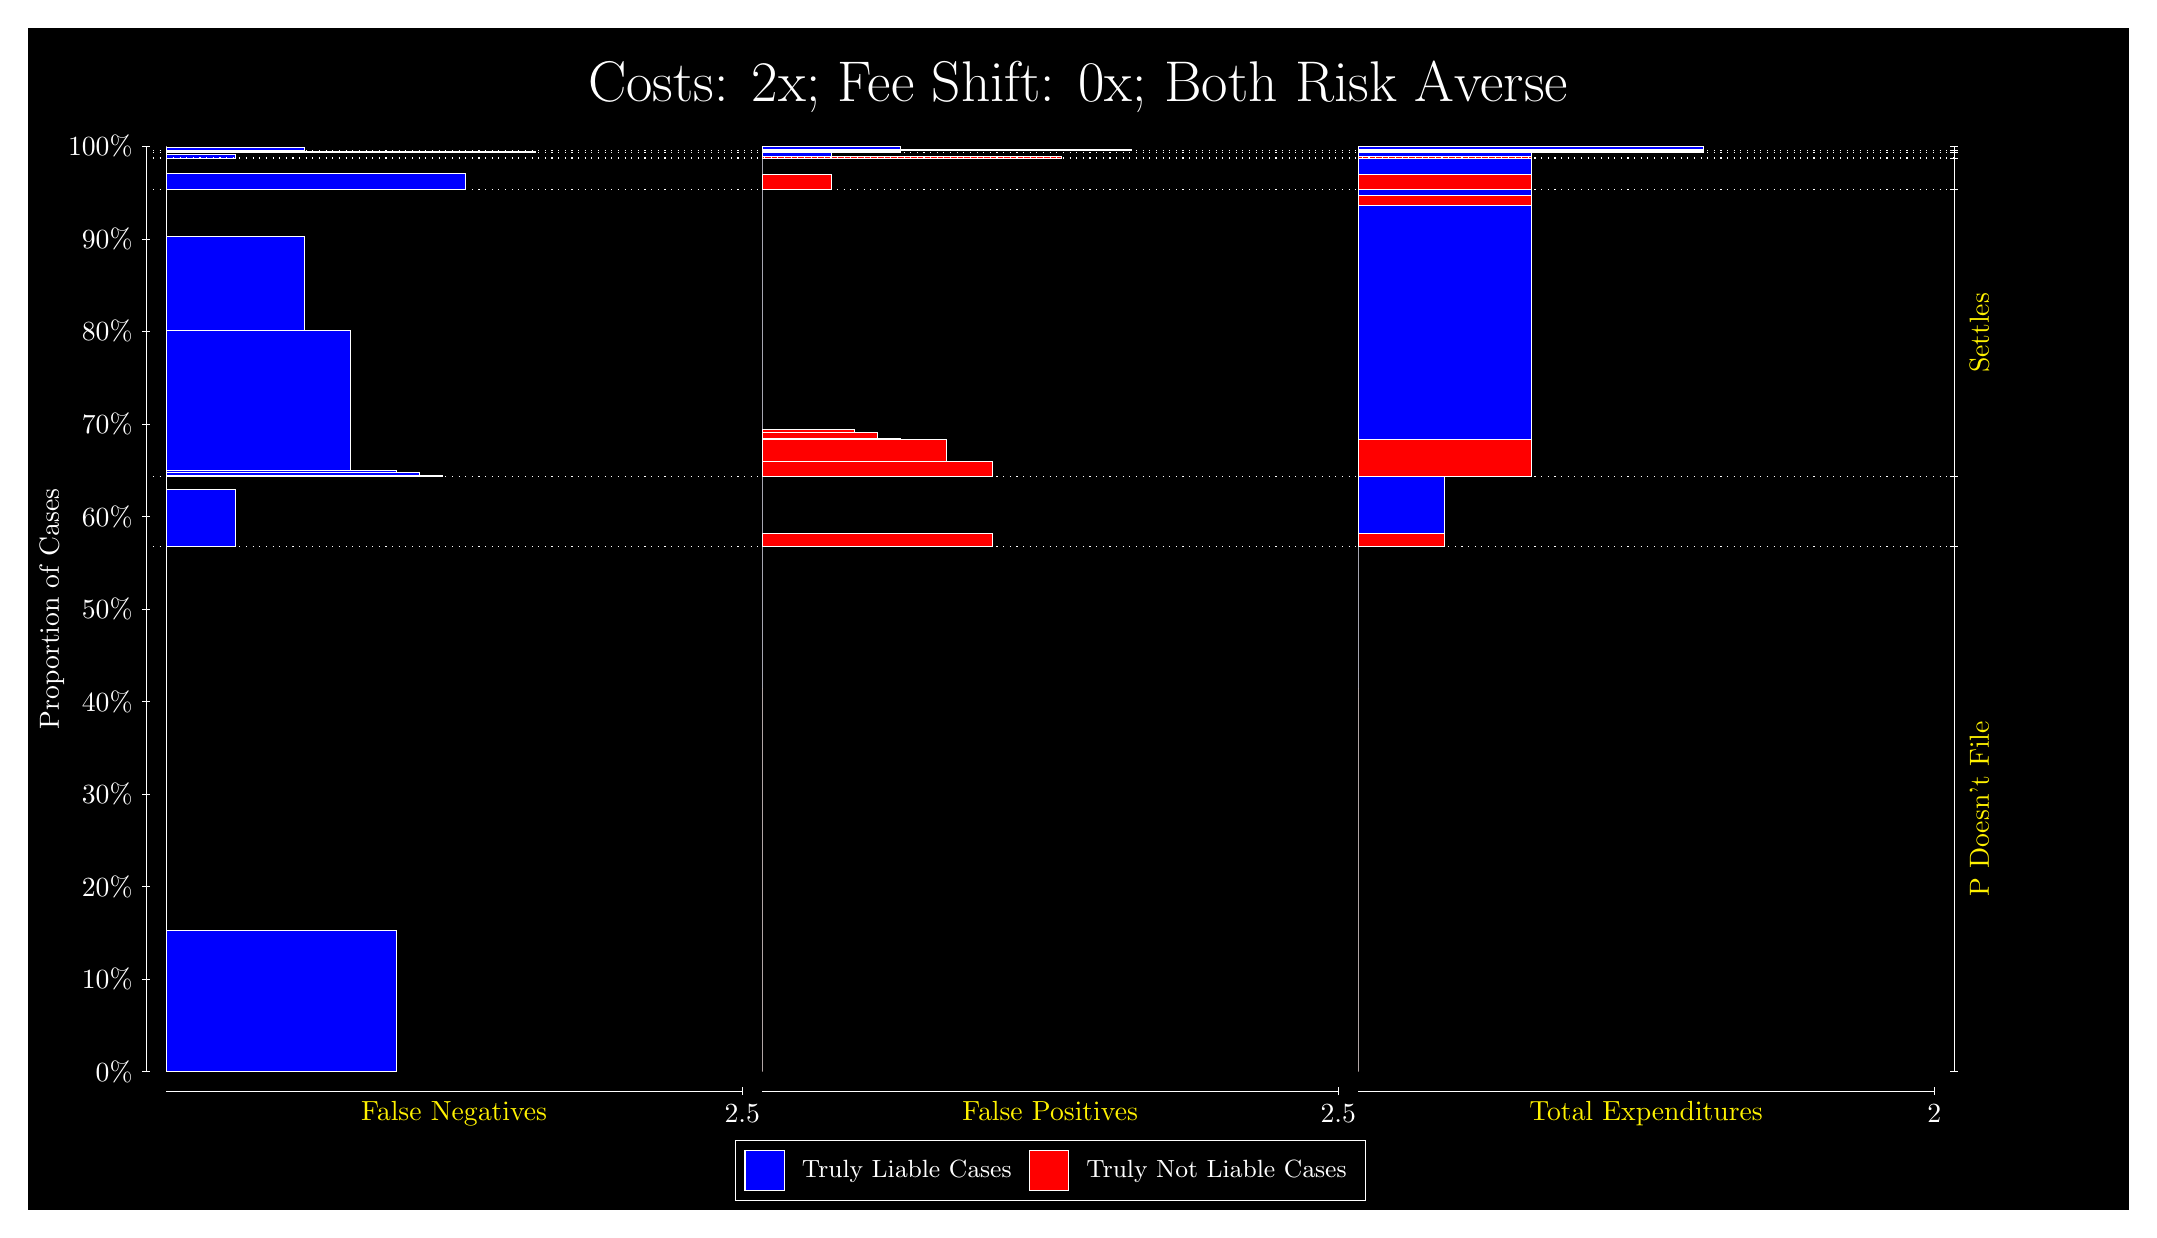
\begin{tikzpicture}
\draw[fill=black] (0,0) rectangle (26.667,15);
\draw[text=white] (0,13.5) rectangle (26.667,15) node[midway] {\huge Costs: 2x; Fee Shift: 0x; Both Risk Averse};
\draw[white, very thin] (1.5,1.75) -- (1.5,13.5);
\node[rotate=90, text=white, anchor=center] at (0.3, 7.625) {Proportion of Cases};
\draw[white, very thin] (1.45,1.75) -- (1.55,1.75);
\node[text=white, anchor=east] at (1.45, 1.75) {0\%};
\draw[white, very thin] (1.45,2.925) -- (1.55,2.925);
\node[text=white, anchor=east] at (1.45, 2.925) {10\%};
\draw[white, very thin] (1.45,4.1) -- (1.55,4.1);
\node[text=white, anchor=east] at (1.45, 4.1) {20\%};
\draw[white, very thin] (1.45,5.275) -- (1.55,5.275);
\node[text=white, anchor=east] at (1.45, 5.275) {30\%};
\draw[white, very thin] (1.45,6.45) -- (1.55,6.45);
\node[text=white, anchor=east] at (1.45, 6.45) {40\%};
\draw[white, very thin] (1.45,7.625) -- (1.55,7.625);
\node[text=white, anchor=east] at (1.45, 7.625) {50\%};
\draw[white, very thin] (1.45,8.8) -- (1.55,8.8);
\node[text=white, anchor=east] at (1.45, 8.8) {60\%};
\draw[white, very thin] (1.45,9.975) -- (1.55,9.975);
\node[text=white, anchor=east] at (1.45, 9.975) {70\%};
\draw[white, very thin] (1.45,11.15) -- (1.55,11.15);
\node[text=white, anchor=east] at (1.45, 11.15) {80\%};
\draw[white, very thin] (1.45,12.325) -- (1.55,12.325);
\node[text=white, anchor=east] at (1.45, 12.325) {90\%};
\draw[white, very thin] (1.45,13.5) -- (1.55,13.5);
\node[text=white, anchor=east] at (1.45, 13.5) {100\%};

\draw[white, very thin] (24.457,1.75) -- (24.457,13.5);
\draw[white, very thin] (24.407,1.75) -- (24.507,1.75);
\node[anchor=west] at (24.407, 1.75) {};
\draw[white, very thin] (24.407,8.4205) -- (24.507,8.4205);
\node[anchor=west] at (24.407, 8.4205) {};
\draw[white, very thin] (24.407,9.3124) -- (24.507,9.3124);
\node[anchor=west] at (24.407, 9.3124) {};
\draw[white, very thin] (24.407,12.949) -- (24.507,12.949);
\node[anchor=west] at (24.407, 12.949) {};
\draw[white, very thin] (24.407,13.352) -- (24.507,13.352);
\node[anchor=west] at (24.407, 13.352) {};
\draw[white, very thin] (24.407,13.419) -- (24.507,13.419);
\node[anchor=west] at (24.407, 13.419) {};
\draw[white, very thin] (24.407,13.446) -- (24.507,13.446);
\node[anchor=west] at (24.407, 13.446) {};
\draw[white, very thin] (24.407,13.5) -- (24.507,13.5);
\node[anchor=west] at (24.407, 13.5) {};

\draw[white, very thin, fill=blue] (1.75,1.75) rectangle (4.6775,3.5502);
\draw[white, very thin, fill=red] (1.75,3.5502) rectangle (1.75,8.4205);
\draw[white, very thin, fill=blue] (1.75,8.4205) rectangle (2.6283,9.1481);
\draw[white, very thin, fill=red] (1.75,9.1481) rectangle (1.75,9.3124);
\draw[white, very thin, fill=blue] (1.75,9.3124) rectangle (5.2631,9.322);
\draw[white, very thin, fill=blue] (1.75,9.322) rectangle (4.9703,9.3644);
\draw[white, very thin, fill=blue] (1.75,9.3644) rectangle (4.6775,9.3803);
\draw[white, very thin, fill=blue] (1.75,9.3803) rectangle (4.092,11.164);
\draw[white, very thin, fill=blue] (1.75,11.164) rectangle (3.5065,12.353);
\draw[white, very thin, fill=red] (1.75,12.353) rectangle (1.75,12.949);
\draw[white, very thin, fill=blue] (1.75,12.949) rectangle (5.5558,13.158);
\draw[white, very thin, fill=red] (1.75,13.158) rectangle (1.75,13.352);
\draw[white, very thin, fill=blue] (1.75,13.352) rectangle (2.6283,13.396);
\draw[white, very thin, fill=red] (1.75,13.396) rectangle (1.75,13.419);
\draw[white, very thin, fill=blue] (1.75,13.419) rectangle (6.4341,13.431);
\draw[white, very thin, fill=red] (1.75,13.431) rectangle (1.75,13.446);
\draw[white, very thin, fill=blue] (1.75,13.446) rectangle (3.5065,13.488);
\draw[white, very thin, fill=red] (1.75,13.488) rectangle (1.75,13.5);
\draw[white, very thin, fill=red] (9.3189,1.75) rectangle (9.3189,6.6203);
\draw[white, very thin, fill=blue] (9.3189,6.6203) rectangle (9.3189,8.4205);
\draw[white, very thin, fill=red] (9.3189,8.4205) rectangle (12.246,8.5849);
\draw[white, very thin, fill=blue] (9.3189,8.5849) rectangle (9.3189,9.3124);
\draw[white, very thin, fill=red] (9.3189,9.3124) rectangle (12.246,9.4972);
\draw[white, very thin, fill=red] (9.3189,9.4972) rectangle (11.661,9.7743);
\draw[white, very thin, fill=red] (9.3189,9.7743) rectangle (11.075,9.7864);
\draw[white, very thin, fill=red] (9.3189,9.7864) rectangle (10.783,9.8631);
\draw[white, very thin, fill=red] (9.3189,9.8631) rectangle (10.49,9.9085);
\draw[white, very thin, fill=blue] (9.3189,9.9085) rectangle (9.3189,12.949);
\draw[white, very thin, fill=red] (9.3189,12.949) rectangle (10.197,13.142);
\draw[white, very thin, fill=blue] (9.3189,13.142) rectangle (9.3189,13.352);
\draw[white, very thin, fill=red] (9.3189,13.352) rectangle (13.125,13.376);
\draw[white, very thin, fill=blue] (9.3189,13.376) rectangle (10.197,13.419);
\draw[white, very thin, fill=red] (9.3189,13.419) rectangle (11.075,13.434);
\draw[white, very thin, fill=blue] (9.3189,13.434) rectangle (9.3189,13.446);
\draw[white, very thin, fill=red] (9.3189,13.446) rectangle (14.003,13.459);
\draw[white, very thin, fill=blue] (9.3189,13.459) rectangle (11.075,13.5);
\draw[white, very thin, fill=red] (16.888,1.75) rectangle (16.888,6.6203);
\draw[white, very thin, fill=blue] (16.888,6.6203) rectangle (16.888,8.4205);
\draw[white, very thin, fill=red] (16.888,8.4205) rectangle (17.986,8.5849);
\draw[white, very thin, fill=blue] (16.888,8.5849) rectangle (17.986,9.3124);
\draw[white, very thin, fill=red] (16.888,9.3124) rectangle (19.083,9.7743);
\draw[white, very thin, fill=blue] (16.888,9.7743) rectangle (19.083,12.747);
\draw[white, very thin, fill=red] (16.888,12.747) rectangle (19.083,12.881);
\draw[white, very thin, fill=blue] (16.888,12.881) rectangle (19.083,12.949);
\draw[white, very thin, fill=red] (16.888,12.949) rectangle (19.083,13.142);
\draw[white, very thin, fill=blue] (16.888,13.142) rectangle (19.083,13.352);
\draw[white, very thin, fill=red] (16.888,13.352) rectangle (19.083,13.376);
\draw[white, very thin, fill=blue] (16.888,13.376) rectangle (19.083,13.419);
\draw[white, very thin, fill=red] (16.888,13.419) rectangle (21.279,13.434);
\draw[white, very thin, fill=blue] (16.888,13.434) rectangle (21.279,13.446);
\draw[white, very thin, fill=red] (16.888,13.446) rectangle (21.279,13.459);
\draw[white, very thin, fill=blue] (16.888,13.459) rectangle (21.279,13.5);
\draw[white, dotted] (1.5,8.4205) -- (24.457,8.4205);
\draw[white, dotted] (1.5,9.3124) -- (24.457,9.3124);
\draw[white, dotted] (1.5,12.949) -- (24.457,12.949);
\draw[white, dotted] (1.5,13.352) -- (24.457,13.352);
\draw[white, dotted] (1.5,13.419) -- (24.457,13.419);
\draw[white, dotted] (1.5,13.446) -- (24.457,13.446);
\draw[white, very thin] (1.75,1.5) -- (9.0689,1.5);
\node[text=yellow, anchor=north] at (5.4094, 1.5) {False Negatives};
\draw[white, very thin] (9.0689,1.45) -- (9.0689,1.55);
\node[text=white, anchor=north] at (9.0689, 1.45) {2.5};

\draw[white, very thin] (9.3189,1.5) -- (16.638,1.5);
\node[text=yellow, anchor=north] at (12.978, 1.5) {False Positives};
\draw[white, very thin] (16.638,1.45) -- (16.638,1.55);
\node[text=white, anchor=north] at (16.638, 1.45) {2.5};

\draw[white, very thin] (16.888,1.5) -- (24.207,1.5);
\node[text=yellow, anchor=north] at (20.547, 1.5) {Total Expenditures};
\draw[white, very thin] (24.207,1.45) -- (24.207,1.55);
\node[text=white, anchor=north] at (24.207, 1.45) {2};

\node[text=yellow, centered, rotate=90] at (24.777, 5.0852) {P Doesn't File};

\node[text=yellow, centered, rotate=90] at (24.777, 11.131) {Settles};





\draw (12.978300999999998,1.5) node[draw=none] (baseCoordinate) {};
\begin{scope}[align=center]
        \matrix[scale=0.5, draw=white, below=0.5cm of baseCoordinate, nodes={draw}, column sep=0.1cm]{
            \node[rectangle, draw, minimum width=0.5cm, minimum height=0.5cm, fill=blue] {}; &
            \node[draw=none, font=\small, text=white] (B) {Truly Liable Cases}; &
            \node[rectangle, draw, minimum width=0.5cm, minimum height=0.5cm, fill=red] {}; &
            \node[draw=none, font=\small, text=white] (B) {Truly Not Liable Cases}; \\
            };
\end{scope}

\end{tikzpicture}
\end{document}